\section{Persistent Memtable}

This section presents the design and implementation of our work PC-DB, figure\ref{fig:structure} 


    \begin{figure}
        \centering
        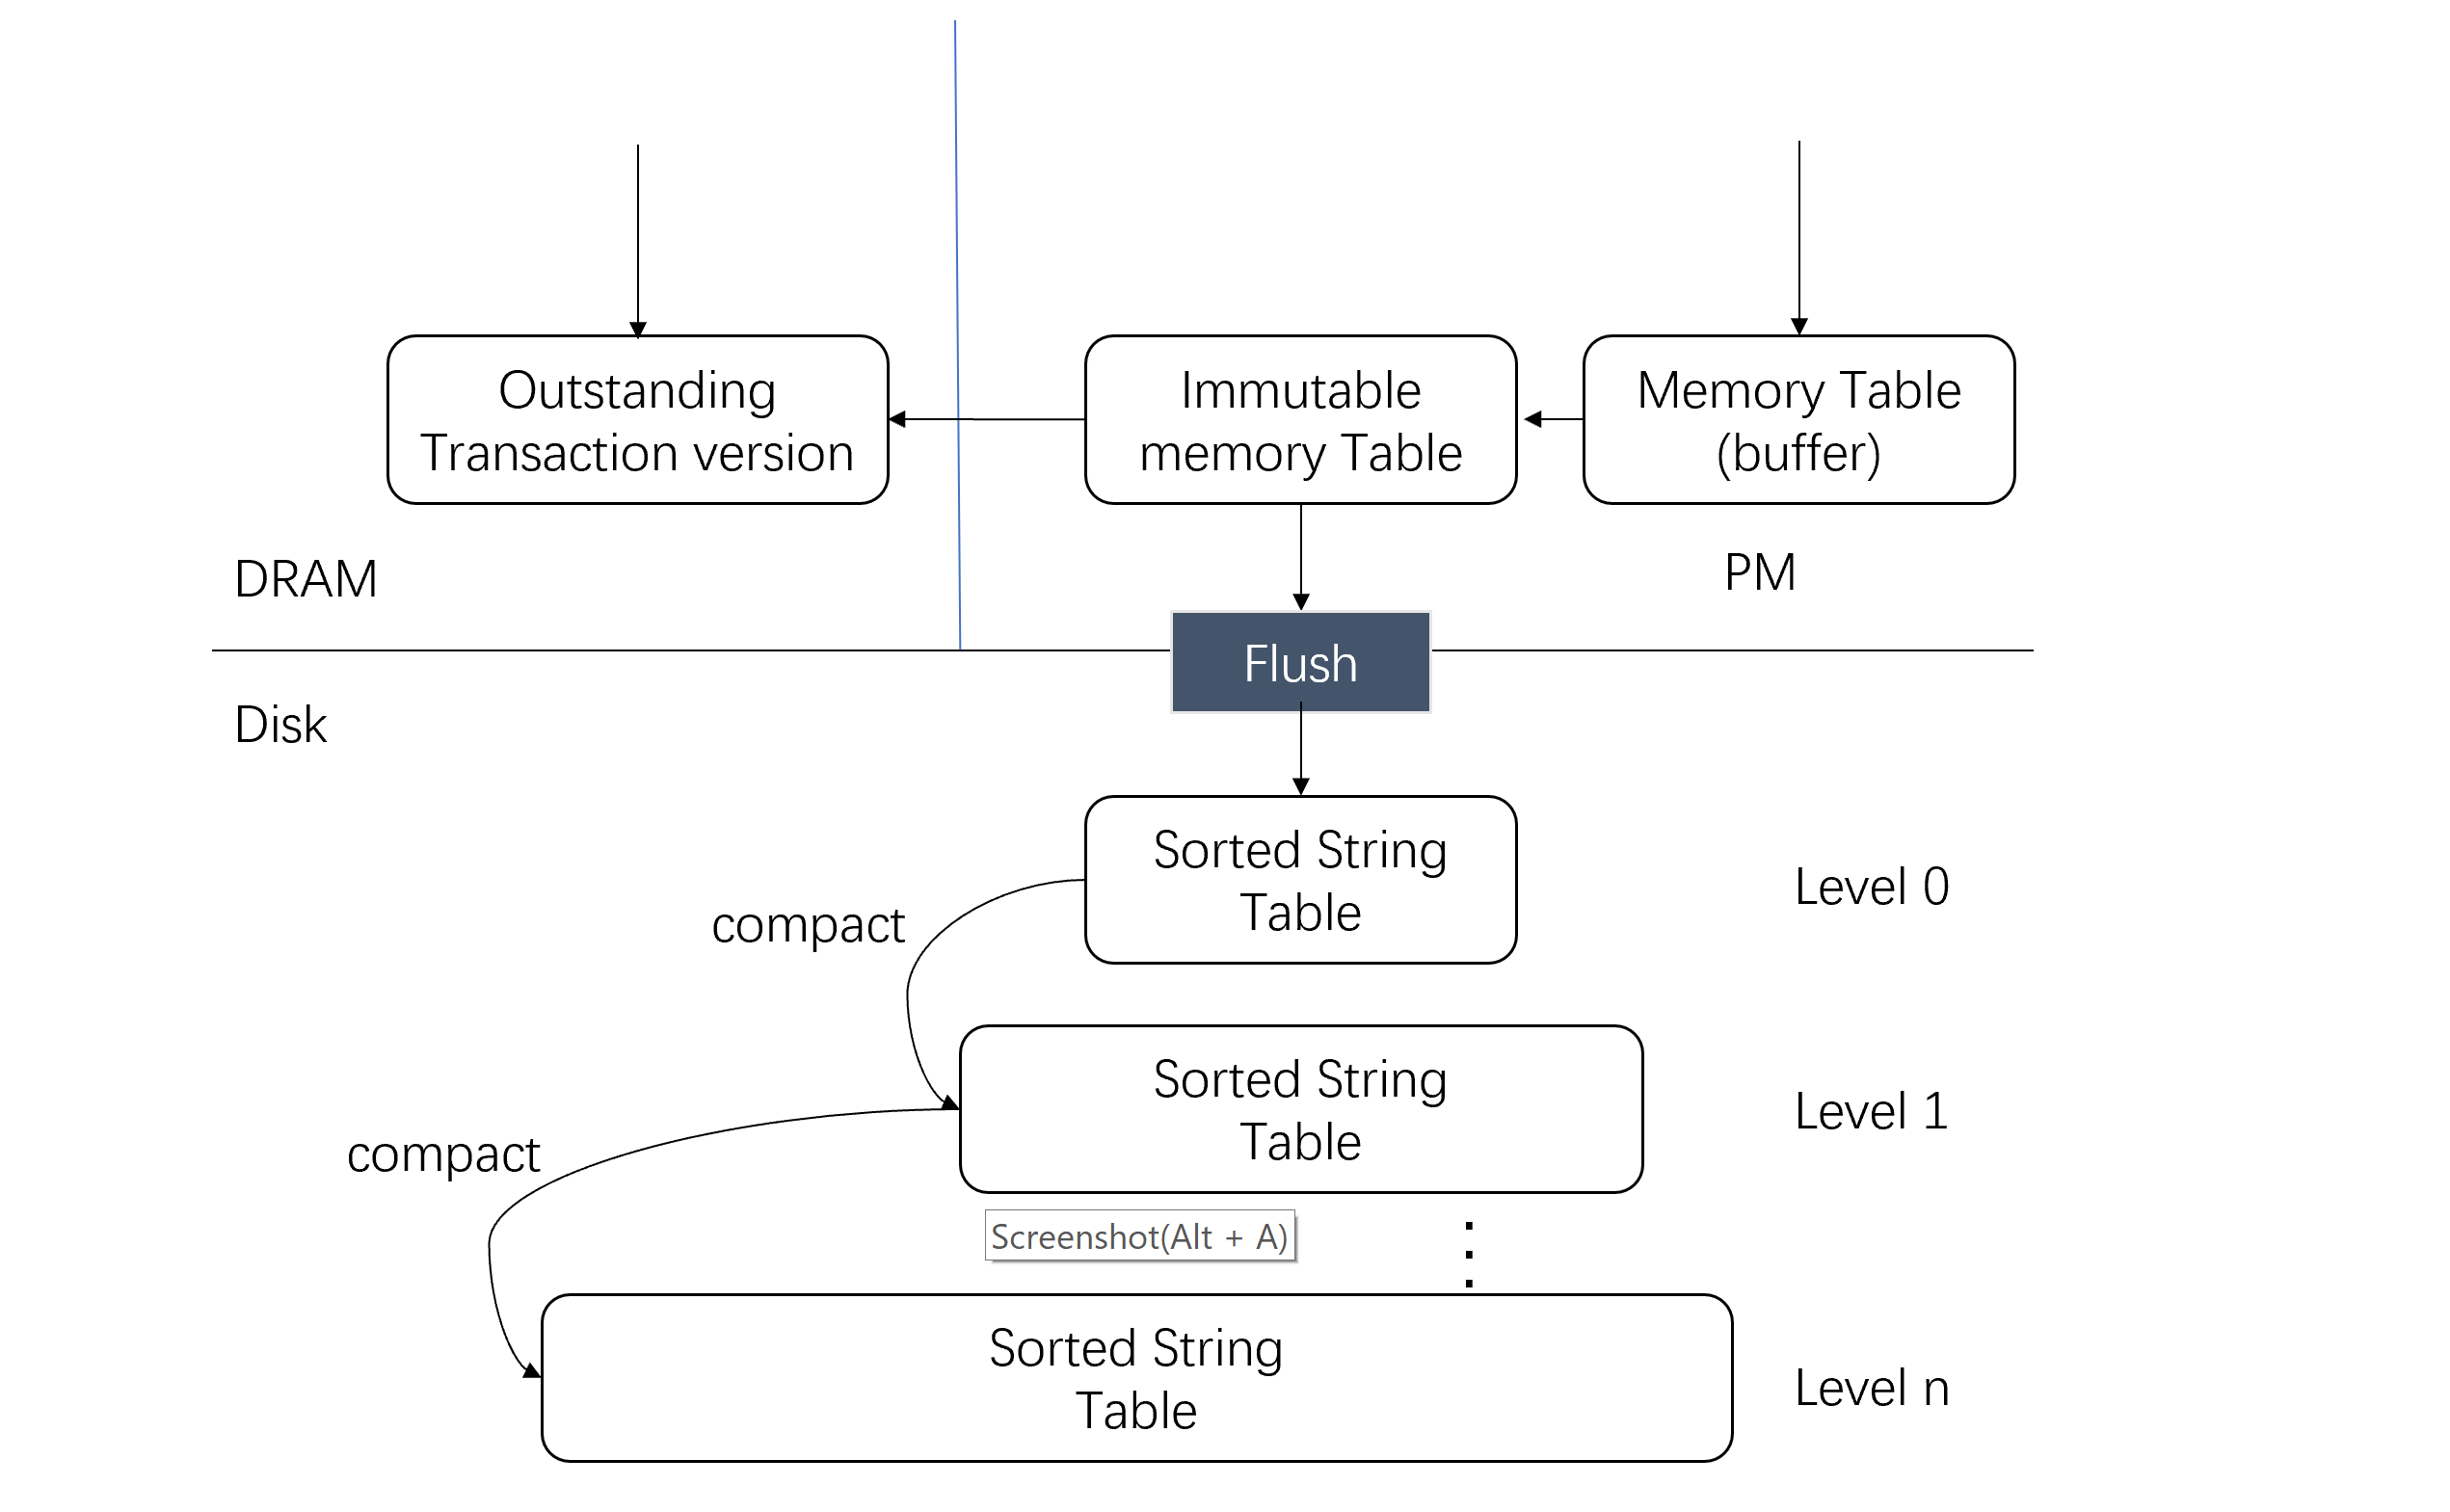
\includegraphics[width=0.36\paperwidth]{figure/structure.png}
        \caption{PC-DB architecture.}
        \label{fig:structure}
    \end{figure}
shows the overall system architecture of PC-DB. 
PC-DB makes a trade-off between the performance and the consistency, it leverages PM to store MemTable and Immutable Memtable. 
In this way, the Memtable and Immutable Memtable are persistent ,thus eliminating the write ahead log(WAL). 
RocksDB ~\cite{RocksDB} by default disables the WAL in order to provide better performance, 
so persistent Memtable and immutable Memtable in PC-DB will provide stronger durability and consistency upon system failures.

RocksDB adopts OCC for transaction serialization.
For OCC, verification of records on disk is slow due to the multiple levels on the disk. 
RocksDB uses the minimum sequence number in memory and global sequence to determine whether to validate in memory. 
If the sequence is not in memory, the transaction will abort to avoid disk access.
In order to optimize the read amplification problem and reduce the probability of transaction abort, 
we use DRAM-based cache to maintain the sequence number of outstanding transactions, 
so that we only need to validate the sequence number in PM and DRAM in the validation phase instead of serching disk.




\subsection{Persistent MemTable}
In Rock-DB, MemTable is a skiplist stored in DRAM, which is not persistent. 
It adopts a Write Ahead Log(WAL) for system consistency.
WAL includes the key -value pairs ,version and checksum,which is sequentially appended in the persistent storage. 
However, the overheads of WAL become the bottleneck of write operations and it takes rather long time to recover from crash since it scans long WAL for recovery.

Based on the above problems, we adopt persistent memory for optimization. 
The Memtable is stored in persistent memory ,which avoids the overheads of WAL for consistency and durability. 
The MemTable is a persistent skiplist, which is the same data structure in  RocksDB. As we have talked before, the PM support atomic writes of 8 bytes, and in the skiplist, operations like inseration, update, and deletion can be done using an atomic 8 bytes write operation.
We adopt  $mfence()$ to achieve instruction serialization and $clflush()$ to guarantee that data in cache is flushed into persistent memory and can be recovered under failure. 
Algorithm 1 shows the insert operation. Other operations such as update and delete can also be achieved by logical insert operation.

To put a KV pair into the PC-DB, PC-DB inserts the KV pair along with its version into the MemTable. When the MemTable is full,it will be treated as an Immutable Memtable. The KV pair will eventually be flushed to an SSTable in $L_0$, 
The KV pair may be compacted and writen to a new SSTable by the compaction of PC-DB, which is the same as RocksDB.


\begin{algorithm}[t]
\caption{Insert(key, value, version,preNode)} %算法的名字


currentNode:=new Node(key,value,version);

mfence();

currentNode.next=preNode.next;

clflush(currentNode);

mfence();

preNode.next:=currentNode;

clflush(preNode.next);

mfence();

\end{algorithm}

Once the system fails, 
the skiplist can be recovered  by locating the root of skiplist, 
the address of which is stored in the MANIFEST file. In the recovery process,the files is also remaped and retrieves the root data structure that stores all pointers to other data structures such as the MemTable and the Immutable MemTable. The PC-DB will also flush the Immutable MemTable if there exits one.
Because the data has already stored in persistent memory,it will be quick compared with recovering from WAL.


\subsection{DRAM-based Cache}
PC-DB uses DRAM as the cache of outstanding transaction version to speed up the version verification in Optimistic Concurrency Control (OCC). This is a space for time strategy.
There are two main methods to mix PM and DRAM memory. The first method is to use DRAM as the cache of PM, and the other method is to use PM and DRAM in parallel,as shown in figure 3. In PC-DB, we choose the second method, which uses DRAM as the cache of outstanding transaction version instead of PM.
\begin{figure}
    \centering
    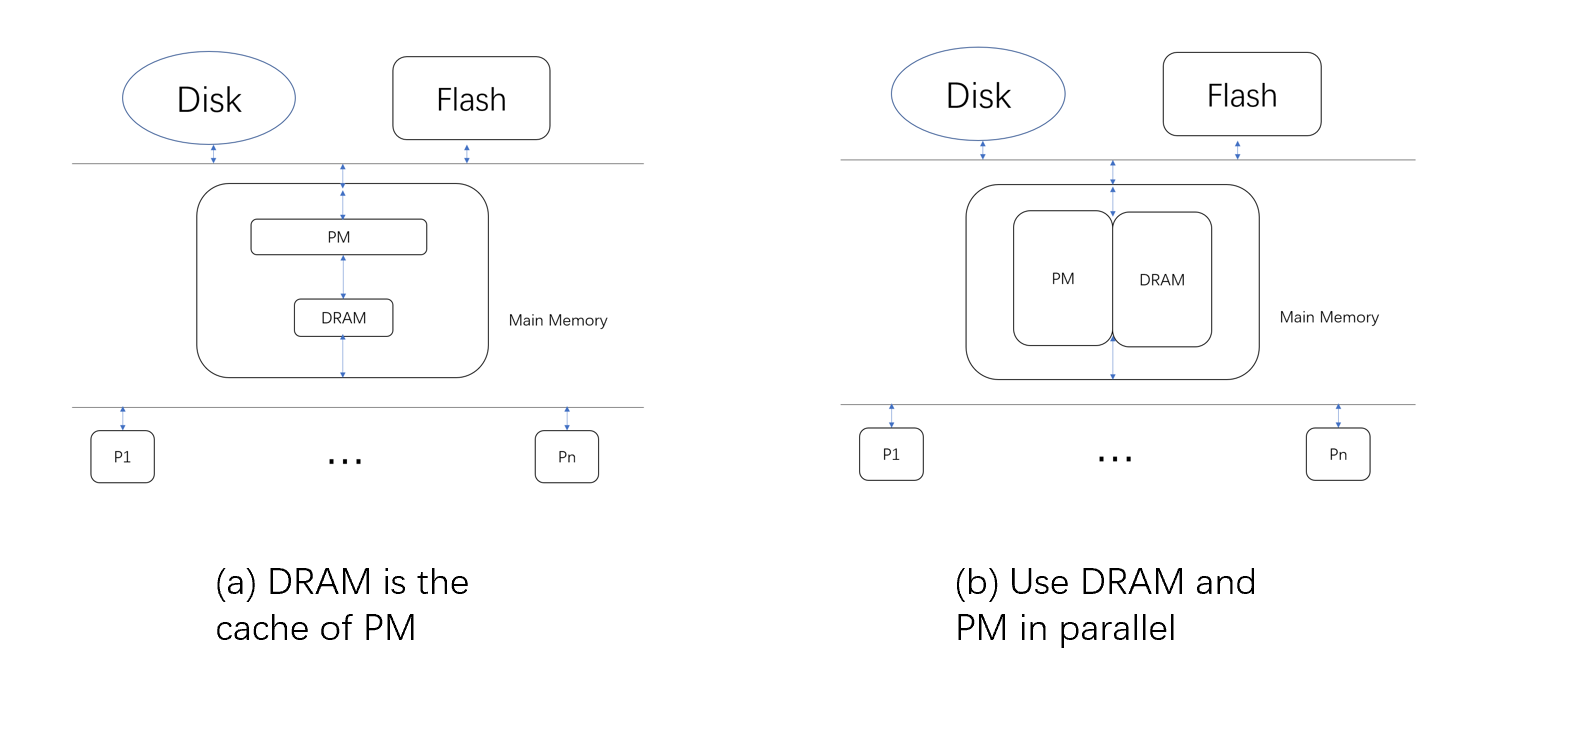
\includegraphics[width=0.36\paperwidth]{USENIX/figure/PM_DRAM.png}
    \caption{Structure of two PM and DRAM mixing methods}
    \label{fig:throughput}
\end{figure}
Take Intel OPTANE DC Persistent Memory\cite{OPTANE} as an example. OPTANE DC Persistent Memory offers two mode: Memory mode and App Direct Mode. When configured to memory mode, application and system sense volatile memory pools. DRAM is used to cache the most frequently accessed data, as well as the PM. It is the first way to mix PM and DRAM. When the App Direct Mode is configured, the application and the operating system clearly know that there are two types of load / storage memory in the platform, and which type of data read / write is suitable for DRAM or Intel OPTANE DC Persistent Memory. Using App Direct Mode, we can store the outstanding transaction version in the DRAM, and use PM to store the MemTable and Immutable MemTable.

Figure 4 shows the algorithm of the Optimistic Concurrency Control of RocksDB. During the commit phase, RocksDB validates the sequence number of each record in the read set. If the latest version of the record does not match the version at the time the record was read, the transaction will abort. There is an observation to introduce the DRAM-based cache: during the commit phase, if the latest version has been flushed into the SSTable, we have to retrieve the record in the SSTable, which will affect the performance due to read amplification. In RocksDB, it maintains the minimal sequence number in the memory, and gets the global sequence number when reading a record. When validating, if the earliest sequence number is smaller than the global sequence number, we only need to validate the version in memory. This approach has some weakness. It will abort some transactions which are legal when the record version has been flushed into the SSTable. There are many approaches to solve this problem. For example, we can attach an index to each record flushed to the disk, but the index will occupy much memory space, which DRAM can't afford. In the OCC optimization, in order to reduce the memory footprint, we do not create an index for each record. What we are concerned with is only the outstanding transaction version, so we can just cache the outstanding transaction version. In PC-DB, DRAM is introduced as the cache. We use the map data structure to store the outstanding transaction version, and we use the App Direct Mode of the Intel OPTANE DC Persistent Memory to store the map in the DRAM. After PC-DB commits a transaction, it should update or add the corresponding records` versions in the DRAM. To validate the version in the read set during the commit phase in OCC, when the version cannot be retrieved in the persistent memory, PC-DB will retrieve  the key in the  DRAM-based cache and obtain the corresponding version if the key exists in the DRAM. However, if the key is not in the DRAM, PC-DB will set the transaction retry after a period of time, and use a background thread to fetch the lasted version of the key from the disk, rather than just abort the transaction. 
\begin{figure}
    \centering
    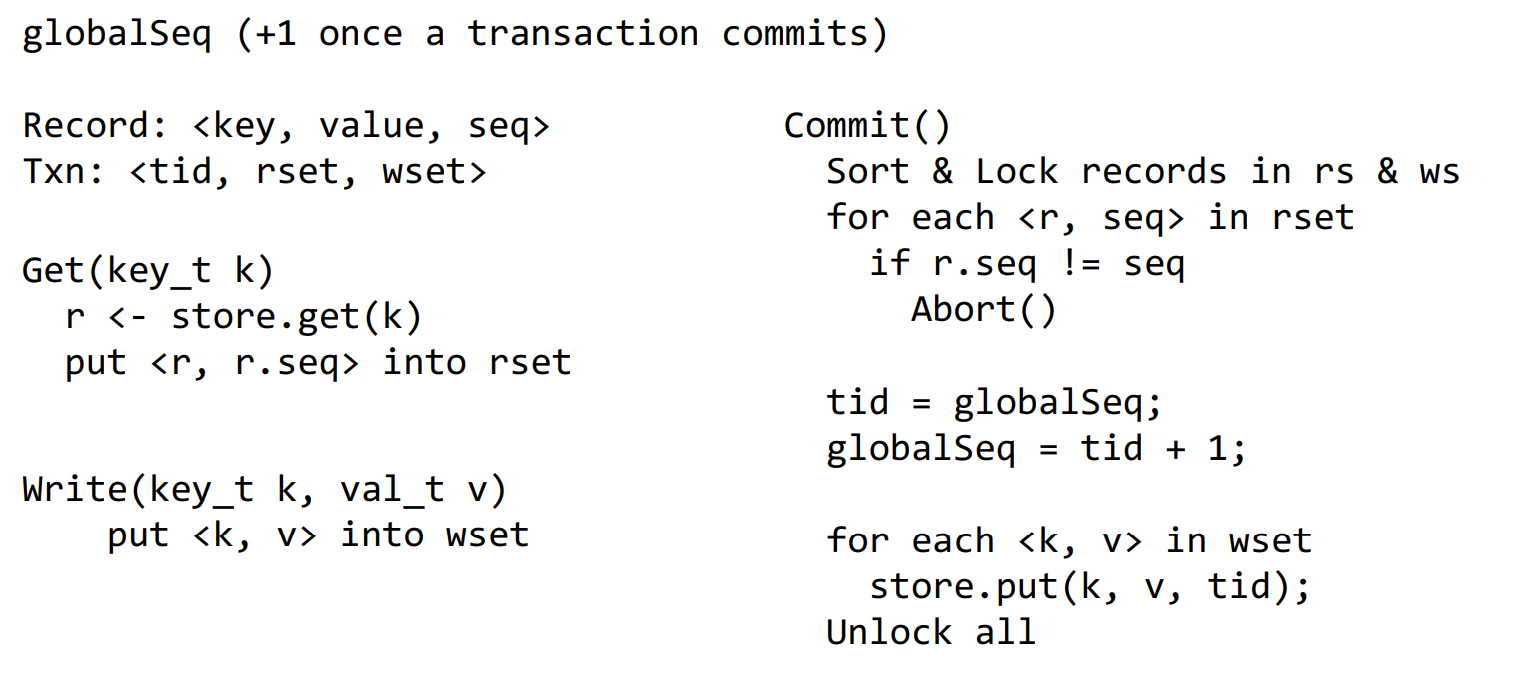
\includegraphics[width=0.36\paperwidth]{USENIX/figure/algorithm.png}
    \caption{Algorithm of the Optimistic Concurrency Control}
    \label{fig:OCCValidation}
\end{figure}
    
\subsection{DRAM Buffer Management}
If PC-DB commits a transaction, it will add the new records' version in the DRAM. Once the DRAM is full, there are several existing strategies to evict the records in the DRAM. One very straight way is to evict the records as soon as the accessing transaction is committed. 
However, if there are other transactions operating on the same records in the meanwhile, they has to wait for the background thread to fetch the versions of the records back to the DRAM, which will take rather a long time. Also, we can  add a reference counter to each of these records in the DRAM. If one transaction makes operations on the record, the reference counter will add one, at the same time, if one transaction is committed, the reference counter of the records it operates on will subtract one. When we need to expel some records, we can evict the records whose reference count is zero. However, this method will transform the read operation into a write operation, which costs a lot. To solve this problem, PC-DB has two approaches. One straight and effective way is to add a valid period for each of the record in the DRAM. When we need to evict some records, we choose these records who are time out. 

Our second approach to evict record is based on the the page swap policy. To manage data buffer, there are many algorithms. The most commonly used algorithm is the LRU algorithm that makes a simple assumption for all the data accesses: if a data block is accessed once, it will be accessed again. This locality metric is also called "recency'', which is implemented by a LRU stack. Each data access is recorded in the LRU stack, where the top entry is the most recent accessed (MRU) and the bottom entry is the least recent accessed (LRU). The LRU entry is the evicted item as the buffer is full (reflected by the full LRU stack). If data access pattern follows the simple assumption of LRU, the strong locality data set is well kept in the buffer by LRU. However, the LRU algorithm fails to handle the following three data access patterns: (1) each data block is only accessed once in a format of sequential scans. In this situation, the buffer would be massively polluted by weak or no locality data blocks. (2) For a cyclic (loop-like) data access pattern, where the loop length is slightly larger than the buffer size, LRU always mistakenly evicts the blocks that will be accessed soon in the next loop. (3) In multiple streams of data accesses where each stream has its own probability for data re-accesses, LRU could not distinguish the probabilities among the streams. 

Our second approach to evict records in the DRAM uses the LIRS algorithm, which performs better than the LRU algorithm. The pages in the DRAM are divided into two kinds: the cold pages and the hot pages. The division is based on the recent operation frequency. When a new record needs to enter into the DRAM but there is no free space, PC-DB chooses a cold page and migrate the page that contains the new records to replace the cold page. In order to divide the pages in DRAM into cold pages and hot pages, LIRS maintains two sets: High Inter-reference Recency set and Low Inter-reference Recency set. Low Inter-reference Recency set contains the pages that are operated on (read and write) frequently within a period of time, While High Inter-reference Recency set contains the cold pages. In the LIRS algorithm, two parameters, IRR(inter-reference recency) and Recency, are used . IRR is the last two visit intervals of a page, and Recency is how many other pages have been visited since the last visit of the page. The IRR and Recency parameters do not contain the number of duplicate pages because the repeated calculation of the page does not have much effect on the priority of current page. The division of High Inter-reference Recency set and Low Inter-reference Recency set is based on the IRR, and if two pages have the same IRR, the page with the larger Recency is replaced. LIRS algorithm use stack S and list Q to manage the two set. Stack S is used to maintain the hot pages and the potential hot pages, and List Q is used to link all the cold pages. In this way, the three LRU issues, which are talked above, are addressed. 
